\documentclass[aspectratio=169, 10pt]{beamer}

% --- Theme & Colors ---
\usetheme{Madrid}
\usecolortheme{dolphin}
\usefonttheme{professionalfonts}

% --- Packages ---
\usepackage{bookmark}
\usepackage{booktabs}
\usepackage{graphicx}
\usepackage{amsmath, amssymb}
\usepackage{hyperref}
\usepackage{ragged2e}
\usepackage{xcolor}
\usepackage{colortbl}

% --- Metadata ---
\title[Musical Carbon Dating]{Musical Carbon Dating}
\subtitle{A Statistical Feature Recognition Approach (1960-2020)}
\author[Group Project]{Group Presentation}
\institute[Data Science]{University Statistical Analysis Project}
\date{\today}

% --- Configuration ---
\setbeamertemplate{navigation symbols}{}
\setbeamerfont{caption}{size=\footnotesize}
\graphicspath{{../output_r/figures/}}

\begin{document}

% -----------------------------------------------------------------------------
% Title Slide
% -----------------------------------------------------------------------------
\begin{frame}
    \titlepage
\end{frame}

% \begin{frame}
%     \centering
%     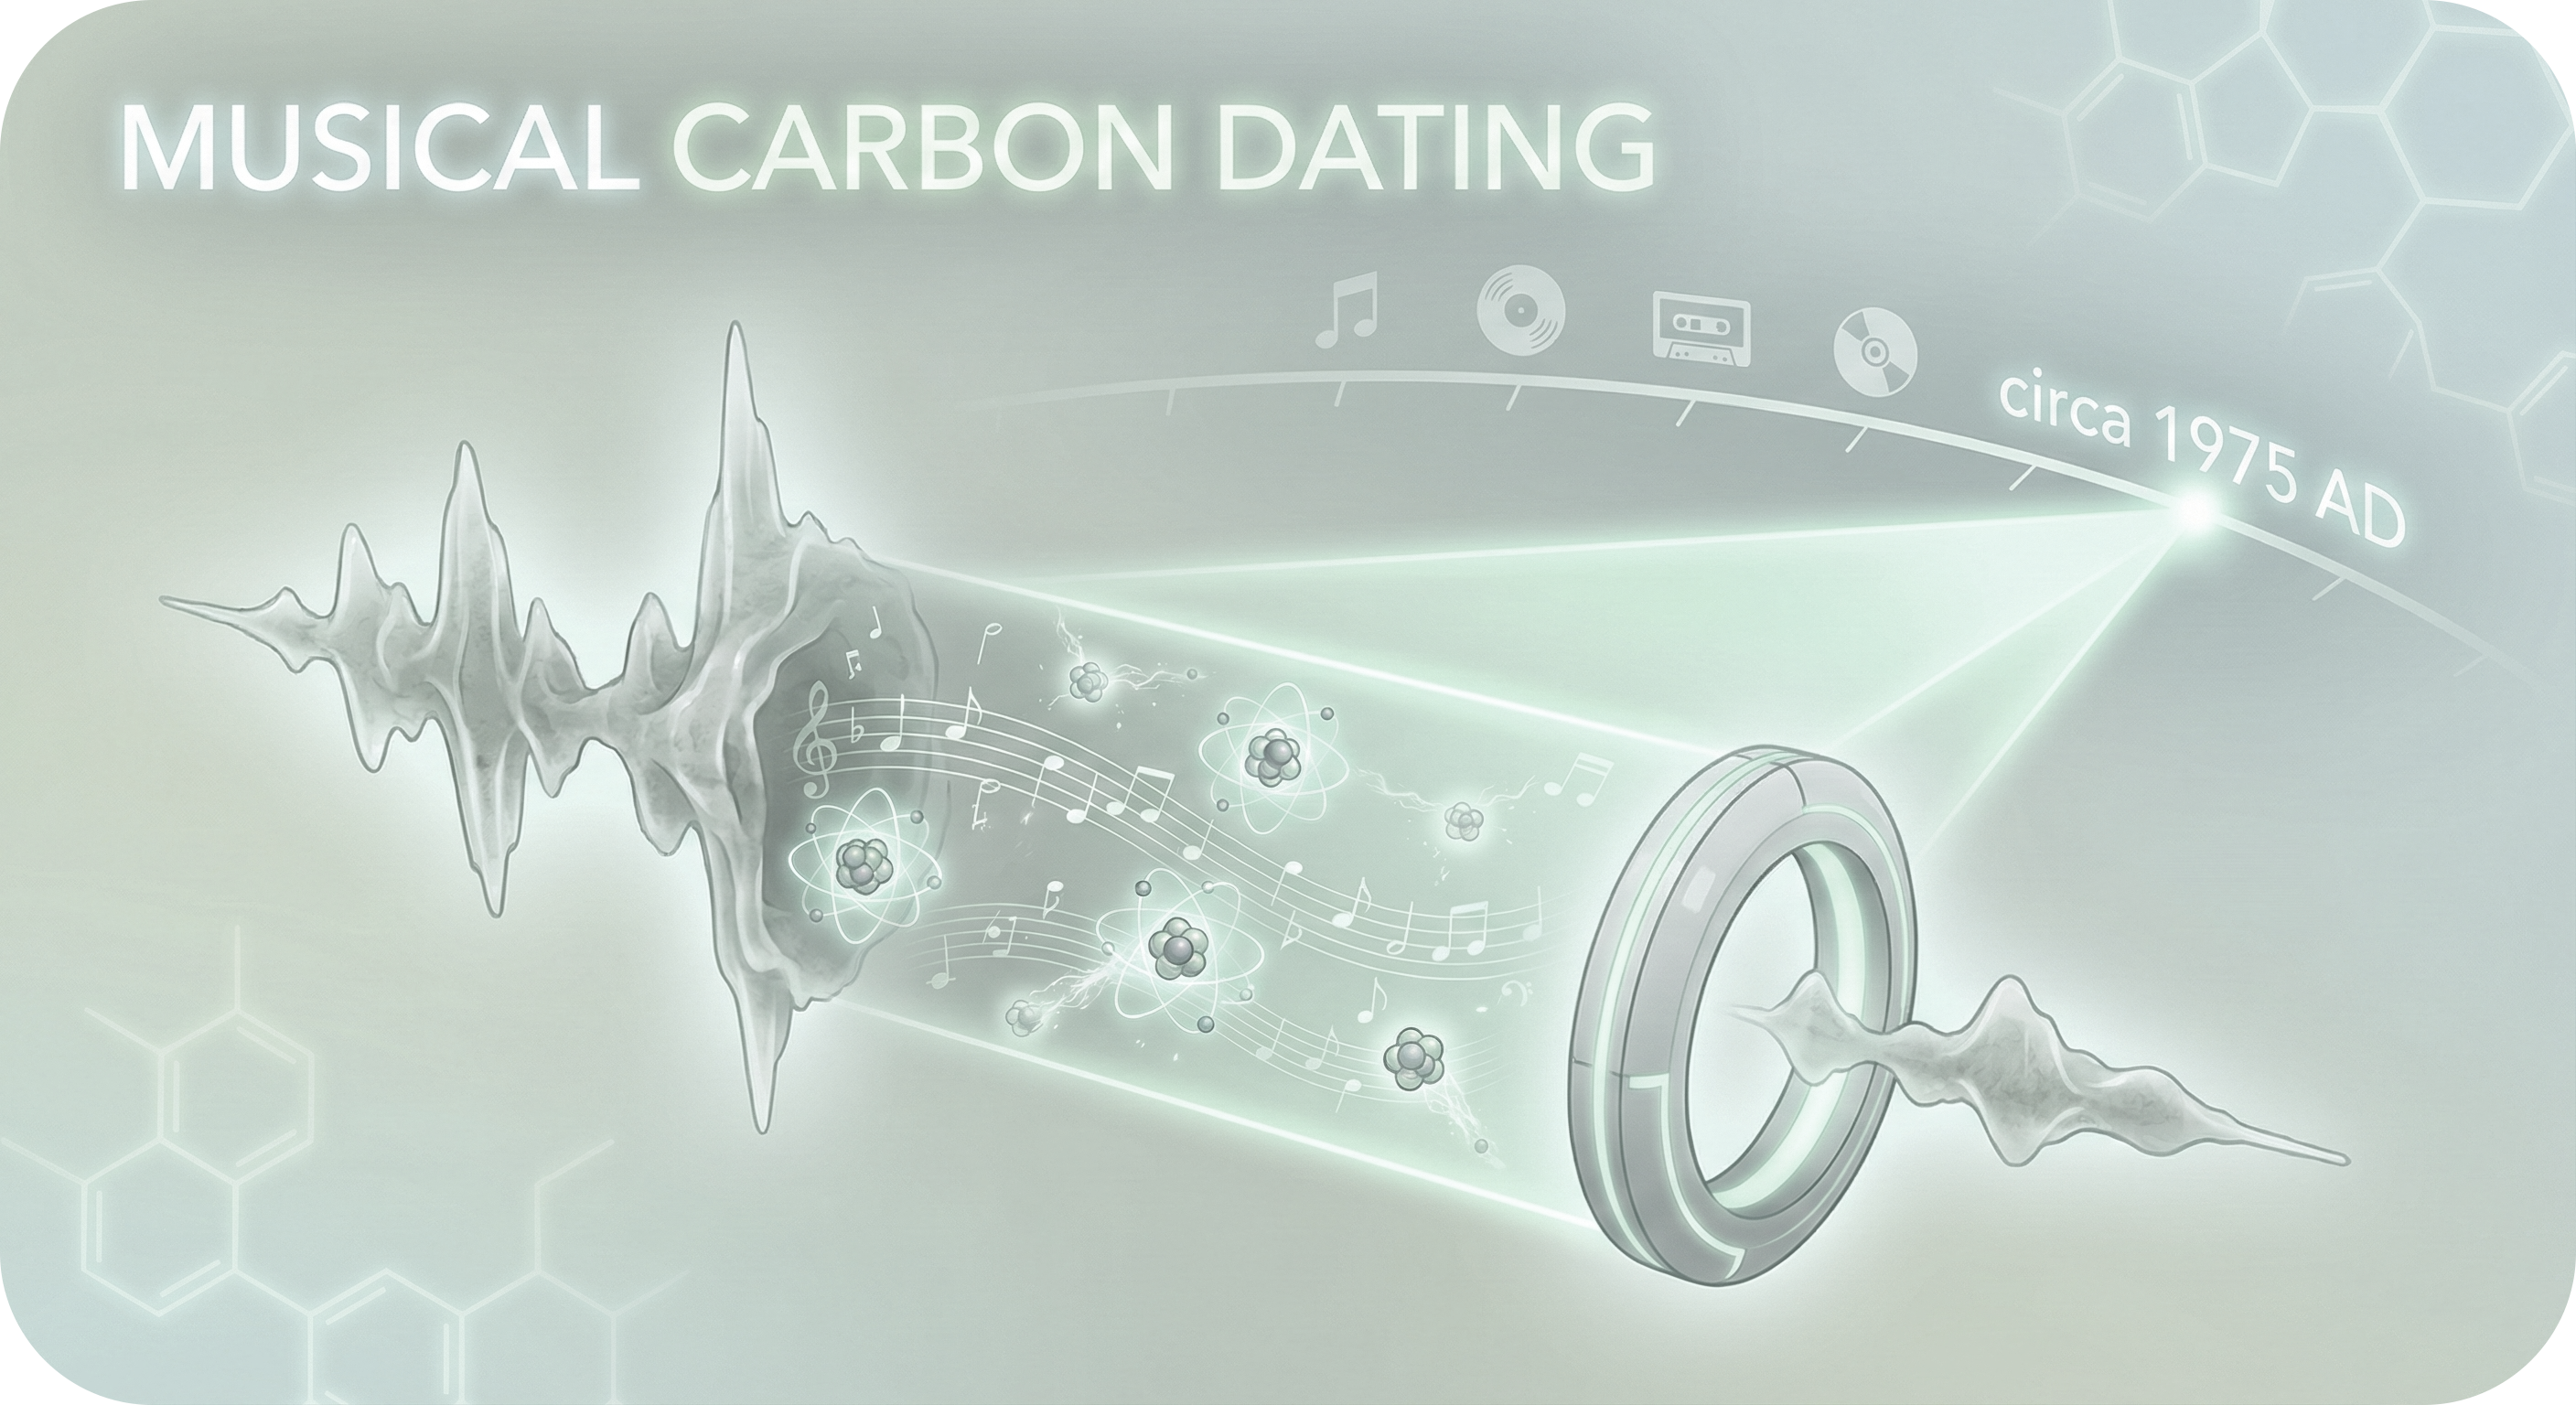
\includegraphics[width=0.9\textwidth]{logo.png}
% \end{frame}

\begin{frame}{Table of Contents}
    \tableofcontents
\end{frame}

% -----------------------------------------------------------------------------
% Section 1: Introduction
% -----------------------------------------------------------------------------
\section{Overview \& Data}

\begin{frame}{The Research Question}
    \begin{block}{Feature Recognition}
        \centering
        \textit{"Can we determine the vintage of a musical recording purely from its acoustic properties?"}
    \end{block}
    
    \vspace{0.5cm}
    \textbf{Objective}: 
    To build a regression model that maps audio features to release year, quantifying the "Arrow of Time" in music production.
    
    \vspace{0.3cm}
    \textbf{Hypothesis}:
    Musical eras have distinct, quantifiable acoustic fingerprints (e.g., the "dryness" of 70s rock vs. the "compression" of 2000s pop).
\end{frame}

\begin{frame}{The Data: Spotify 600k Tracks}
    \textbf{Data Filtering Strategy}:
    \begin{itemize}
        \item \textbf{Source}: Spotify 600k Tracks Dataset (Kaggle).
        \item \textbf{Filter 1}: Timeframe $1960 \le T \le 2020$ (Modern Era).
        \item \textbf{Filter 2}: \texttt{popularity > 30} (Focus on culturally significant music).
        \item \textbf{Final Sample}: $N = \mathbf{250,971}$ tracks (1960--2020).
    \end{itemize}
    
    \vspace{0.5cm}
    \textbf{Validation Strategy}:
    \begin{itemize}
        \item \textbf{Random Split}: 80\% Training / 20\% Test.
        \item \textit{Rationale}: We are testing "feature recognition" (interpolating styles), not future forecasting (extrapolating time).
    \end{itemize}
\end{frame}

\begin{frame}{The Feature Set (p=13)}
    We utilized all 13 available audio features.
    
    \begin{columns}[t]
        \column{0.33\textwidth}
        \textbf{Physical Features}
        \begin{enumerate}
            \item \texttt{Loudness} (dB)
            \item \texttt{Tempo} (BPM)
            \item \texttt{Duration} (ms)
        \end{enumerate}
        
        \column{0.33\textwidth}
        \textbf{Musical Features}
        \begin{enumerate}
            \setcounter{enumi}{3}
            \item \texttt{Key} (0-11)
            \item \texttt{Mode} (Major/Minor)
            \item \texttt{Time Signature}
        \end{enumerate}
        
        \column{0.33\textwidth}
        \textbf{Perceptual Features}
        \begin{enumerate}
            \setcounter{enumi}{6}
            \item \texttt{Acousticness}
            \item \texttt{Danceability}
            \item \texttt{Energy}
            \item \texttt{Instrumentalness}
            \item \texttt{Liveness}
            \item \texttt{Speechiness}
            \item \texttt{Valence} (Positivity)
        \end{enumerate}
    \end{columns}
\end{frame}

% -----------------------------------------------------------------------------
% Section 2: Methodology Pipeline
% -----------------------------------------------------------------------------
\section{Methodology Pipeline}

\begin{frame}{The Regression Pipeline}
    We followed a rigorous 5-phase statistical workflow:
    \vspace{0.5cm}
    \begin{enumerate}
        \item \textbf{Phase I: Simple Linear Regression (SLR)}
        \textit{Hypothesis testing: The "Loudness War".}

        \item \textbf{Data Standardization}
        \textit{Z-Score Normalization ($x' = \frac{x-\mu}{\sigma}$) to ensure scale invariance.}
        
        \item \textbf{Phase II: Multiple Linear Regression (MLR)}
        \textit{Baseline model using all $p=13$ features.}
        
        \item \textbf{Phase III: The Diagnostic Audit} (Critical Step)
        \textit{Testing Linearity, Multicollinearity, Normality, and Homoscedasticity.}
        
        \item \textbf{Phase V: Refinement (WLS)}
        \textit{Weighted Least Squares to correct for Heteroscedasticity.}

        \item \textbf{Phase VI: Interpretation}
        \textit{Quantifying the "Arrow of Time" and Cultural Shifts.}
    \end{enumerate}
\end{frame}

% -----------------------------------------------------------------------------
% Section 3: Analysis
% -----------------------------------------------------------------------------
\section{Phases I--III: Baseline \& Diagnostics}

\begin{frame}{Phase I: The "Loudness War" (SLR)}
    $$ \text{Year}_i = \beta_0 + \beta_{\text{loud}} \cdot \text{Loudness}_i + \varepsilon_i $$
    
    \begin{columns}
        \column{0.5\textwidth}
        \includegraphics[width=1.0\linewidth]{r_feature_trends.png}
        
        \column{0.5\textwidth}
        \textbf{Results}:
        \begin{itemize}
            \item $t$-stat: \textbf{183.3} (Highly Significant).
            \item $\beta_{\text{loud}} \approx 5.44$ years/dB (Standardized).
            \item $R^2 = 0.1434$.
        \end{itemize}
        
        \vspace{0.3cm}
        \textbf{Conclusion}: 
        Tracks have consistently gotten louder, but Loudness alone explains only 14\% of the variance.
    \end{columns}
\end{frame}

\begin{frame}{Phase II: Multiple Linear Regression (Baseline)}
    $$ \mathbf{y} = \mathbf{X}\boldsymbol{\beta} + \boldsymbol{\varepsilon} $$
    
    \begin{itemize}
        \item \textbf{Algorithm}: Ordinary Least Squares (OLS) with all 13 features.
        \item \textbf{Mean Error (MAE)}: 9.72 Years
        \item \textbf{Median Error}: 7.52 Years
    \end{itemize}
    
    \vspace{0.3cm}
    \begin{alertblock}{Why so low?}
       An $R^2$ of 0.14 suggests we are missing non-linear patterns or violating OLS assumptions. We initiated a \textbf{Diagnostic Audit}.
    \end{alertblock}
\end{frame}

\begin{frame}{Phase III: Diagnostic Audit (1/2)}
    \textbf{Test 1: Independence of Errors}
    \begin{itemize}
        \item \textbf{Method}: Durbin-Watson Statistic.
        \item \textbf{Result}: $DW \approx 2.001$. (Target = 2.0)
        \item \textbf{Finding}: \textcolor{green}{Assumption Met.} No autocorrelation. Each song is statistically unique.
    \end{itemize}
    
    \vspace{0.5cm}
    \textbf{Test 2: Multicollinearity}
    \begin{itemize}
        \item \textbf{Method}: Variance Inflation Factor (VIF).
        \item \textbf{Concern}: High correlation between Loudness and Energy ($r=0.74$).
        \item \textbf{Result}: Max VIF (Energy) = \textbf{3.58}. All VIFs $< 5.0$.
        \item \textbf{Finding}: \textcolor{green}{Assumption Met.} No severe multicollinearity.
    \end{itemize}
\end{frame}

\begin{frame}{Phase III: Diagnostic Audit (2/2)}
    \textbf{Test 3: Homoscedasticity (Constant Variance)}
    
    \begin{columns}
        \column{0.5\textwidth}
        \includegraphics[width=1.0\linewidth]{r_error_by_era.png}
        
        \column{0.5\textwidth}
        \begin{itemize}
            \item \textbf{Visual}: Dispersed variance (Right) vs Tight variance (Left).
            \item \textbf{Insight}: "Stylistic Entropy". The definition of specific eras has blurred over time due to technology.
            \item \textbf{Statistic}: $\chi^2 = \mathbf{20,754}$ (Breusch-Pagan).
            \item \textbf{Conclusion}: Variance is expanding. OLS fails because it treats neighboring years inconsistently.
        \end{itemize}
    \end{columns}
    
    \vspace{0.3cm}
    \textbf{Solution}: We must weight the model to trust the "consistent" eras more than the "chaotic" ones. \textbf{Enter WLS.}
\end{frame}

% -----------------------------------------------------------------------------
% Section 4: Solution
% -----------------------------------------------------------------------------
\section{Phases IV--VI: Refinement \& Results}

\begin{frame}{Phase IV: Model Selection}
    We compared two methods to identify the "True" feature set:
    
    \begin{table}[]
        \centering
        \begin{tabular}{lll}
            \toprule
            \textbf{Method} & \textbf{Selected Features} & \textbf{Key Difference} \\
            \midrule
            Stepwise (AIC) & 12 Features & Dropped \texttt{Key} ($p=0.94$) \\
            \rowcolor{green!10} LASSO ($L_1$) & \textbf{12 Features} & \textbf{Corroborated AIC selection} \\
            \bottomrule
        \end{tabular}
    \end{table}
    
    \vspace{0.3cm}
    \textbf{Decision}: We utilized the full acoustic feature set.
    \begin{itemize}
        \item Removing variables offered negligible AIC improvement.
        \item Retaining subtle features (Key, Mode) ensures we capture harmonic evolution.
    \end{itemize}
\end{frame}

\begin{frame}{Phase V: Weighted Least Squares (WLS)}
    To cure Heteroscedasticity, we implemented WLS:
    $$ \min_{\boldsymbol{\beta}} \sum_{i=1}^{n} w_i (y_i - \mathbf{x}_i^T \boldsymbol{\beta})^2, \quad \text{where } w_i \propto \frac{1}{\text{Var}(\varepsilon_i)} $$
    
    \begin{columns}
        \column{0.5\textwidth}
        \centering
        \includegraphics[width=1.0\linewidth]{r_wls_pred_vs_act_v1.png}
    
        \column{0.5\textwidth}
        \begin{alertblock}{What WLS Fixes}
            \begin{itemize}
                \item \textbf{Valid p-values} \& CIs.
                \item \textbf{Efficient coefficients}.
            \end{itemize}
        \end{alertblock}
        
        \vspace{0.1cm}
        \begin{itemize}
            \item Baseline SLR achieves $R^2 = \mathbf{0.14}$
            \item Loudness coefficient: $\beta \approx \mathbf{5.44}$ years/dB
            \item Weighted $R^2$: \textbf{0.26}
            \item Chisquare $\approx \mathbf{20,754}$ ($p < 0.001$)
            \item Test $R^2$: $\approx 0.26$
            \item RMSE: 12.83 yrs
        \end{itemize}
    \end{columns}
    
    \vspace{0.2cm}
    \footnotesize{\textit{Note: The weighted $R^2$ of 0.26 reflects the model's reliability after accounting for heteroscedasticity, maintaining predictive parity with the baseline OLS while ensuring valid inference.}}
\end{frame}

\begin{frame}{Phase VI-A: Technological Drivers ("The Sound of Efficiency")}
    \textbf{Regression reveals the impact of technology on composition ($p < 0.001$).}
    
    \begin{itemize}
        \item \textbf{The Loudness-Energy Paradox (Multicollinearity Insight)}:
        \begin{itemize}
            \item Mean \texttt{Loudness} has skyrocketed ($\beta_{\text{loud}} \approx +7.57$).
            \item Yet, \texttt{Energy}'s coefficient is \textbf{negative} ($\beta_{\text{energy}} \approx -2.05$).
            \item \textbf{Interpretation}: Loudness comes from compression, not composition.
        \end{itemize}

        \item \textbf{The Attention Economy (Duration)}:
        \begin{itemize}
            \item Coefficient $\beta_{\text{duration}} \approx -0.33$ (Negative).
            \item Songs are getting statistically shorter, likely driven by streaming incentives and skipping behavior.
        \end{itemize}
        
        \item \textbf{Instrumentalness} ($\beta \approx +0.20$):
        \small{A shift towards beat-driven (Hip-Hop/EDM) production over vocal-centric ballads.}
    \end{itemize}
\end{frame}

\begin{frame}{Phase VI-B: Cultural Evolution ("The Mood of an Era")}
    \textbf{Applying Statistical Inference to Cultural Theory.}
    
    \begin{itemize}
        \item \textbf{The "Sad Banger" Phenomenon}:
        \begin{itemize}
            \item \textbf{Danceability} ($\beta \approx +3.60$): The single strongest predictor. Rhythm is the defining feature of modernity.
            \item \textbf{Valence} ($\beta \approx -3.39$): Optimism has collapsed.
            \item \textbf{Synthesis}: We are dancing more, but feeling less.
        \end{itemize}

        \item \textbf{The Acousticness Paradox (Ceteris Paribus)}:
        \begin{itemize}
            \item Raw Correlation: Negative ($r \approx -0.12$).
            \item WLS Coefficient: \textbf{Positive} ($\beta \approx +0.65$).
            \item \textbf{Discovery}: \textit{Controlling for Loudness}, modern music actually retains significant acoustic elements (Indie, Lo-Fi), hidden by the "Wall of Sound".
        \end{itemize}
    \end{itemize}
    
    \begin{alertblock}{Analytical Triumph}
       By using \textbf{Partial Regression Coefficients}, we uncovered trends (like the Acousticness reversal) that simple correlation would have missed.
    \end{alertblock}
\end{frame}

% -----------------------------------------------------------------------------
% Section 5: Applications
% -----------------------------------------------------------------------------
\section{Applications}

\begin{frame}{The Nostalgia Index}
    \textit{"One man's error is another man's feature."}
    
    We define the \textbf{Nostalgia Index} as the model's prediction error:
    $$ \text{Index} = | \hat{Y}_{\text{predicted}} - Y_{\text{actual}} | $$
    
    High index = A song that "sounds" like it belongs to a different era.
    
    \begin{columns}
        \column{0.5\textwidth}
        \centering
        \includegraphics[width=1.0\linewidth]{r_nostalgia_distribution.png}
        
        \column{0.5\textwidth}
        \textbf{Distribution Stats}:
        \begin{itemize}
            \item Mean: \textbf{9.72} yrs
        \item Median: \textbf{7.52} yrs
        \item Max: \textbf{85.34} yrs
        \end{itemize}
        
        \vspace{0.2cm}
        \small{The index measures the "stylistic distance" between a song's audio and its true era.}
    \end{columns}
\end{frame}

\begin{frame}{Validation: Detecting "Time Travelers"}
    We validated the index on tracks known for their retro aesthetic.
    
    \begin{table}[]
        \centering
        \small
        \begin{tabular}{ll ccc}
            \toprule
            \textbf{Song} & \textbf{Year} & \textbf{Predicted} & \textbf{Index} & \textbf{Diagnosis} \\
            \midrule
            \textit{Uptown Funk} (Ronson) & 2015 & 2013.1 & \textbf{1.9} & Modern Construction \\
            \rowcolor{yellow!20} \textit{Physical} (Dua Lipa) & 2020 & 2009.0 & \textbf{11.0} & \textbf{Retro Aesthetic} \\
            \rowcolor{red!10} \textit{Blinding Lights} (Weeknd) & 2019 & 2004.2 & \textbf{14.8} & \textbf{80s Revival} \\
            \bottomrule
        \end{tabular}
    \end{table}
    
    \vspace{0.3cm}
    \textbf{Conclusion}: The model correctly identifies these hits as "sounding old", proving it captures aesthetic style rather than just release dates.
\end{frame}

\begin{frame}{Conclusion}
    \begin{enumerate}
        \item \textbf{Recognition}: We can date music to within 7.5 years (median) purely from audio.
        \item \textbf{Rigor}: Diagnostics proved OLS insufficient; WLS corrected the inference.
        \item \textbf{Insight}: Musical evolution is quantifiable and technology-driven.
        \item \textbf{Value}: The Nostalgia Index provides a metric for "Retro-vibe".
    \end{enumerate}
\end{frame}

\begin{frame}
    \centering
    \Huge \textcolor{blue!70!black}{Thank You.}
    
    \vspace{1cm}
\end{frame}

\end{document}

